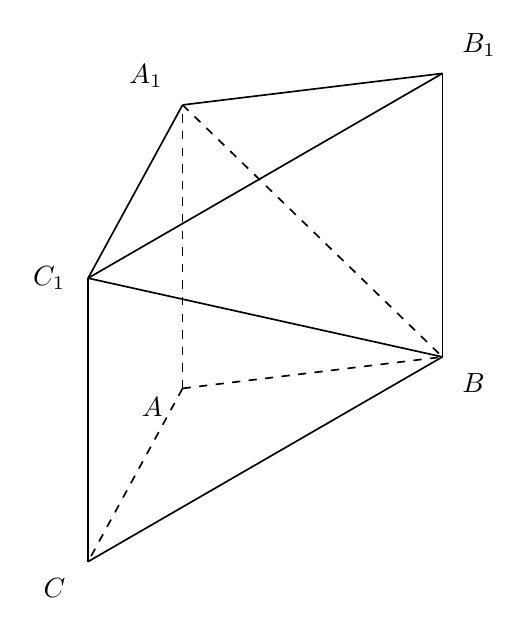
\begin{tikzpicture}[x=1cm,y=1cm,font=\normalsize,
  geometry edge/.style={solid,line width=.6pt,draw=black},
  geometry label/.style={font=\normalsize,inner sep=2pt}]

\coordinate (A) at (1.2,0);
\coordinate (B) at (4.5,0.4);
\coordinate (C) at (0,-2.2);
\coordinate (Aone) at (1.2,3.6);
\coordinate (Bone) at (4.5,4.0);
\coordinate (Cone) at (0,1.4);
\draw[geometry edge] (Cone)--(C);
\draw[geometry edge] (Bone)--(B);
\draw[geometry edge] (Cone)--(C);
\draw[geometry edge] (B)--(C);
\draw[geometry edge] (Cone)--(Aone);
\draw[geometry edge] (Aone)--(Bone);
\draw[geometry edge] (Cone)--(Bone);
\draw[geometry edge] (Cone)--(B);
\draw[geometry edge,dashed] (A)--(B);
\draw[geometry edge,dashed] (A)--(C);
\draw[geometry edge,dashed] (A)--(Aone);
\draw[geometry edge,dashed] (Aone)--(B);
\node[geometry label,below left,xshift=-5pt,yshift=-1pt] at (A) {$A$};
\node[geometry label,below right,xshift=5pt,yshift=-4pt] at (B) {$B$};
\node[geometry label,below left,xshift=-6pt,yshift=-4pt] at (C) {$C$};
\node[geometry label,above left,xshift=-5pt,yshift=4pt] at (Aone) {$A_{1}$};
\node[geometry label,above right,xshift=5pt,yshift=4pt] at (Bone) {$B_{1}$};
\node[geometry label,left,xshift=-6pt] at (Cone) {$C_{1}$};
\end{tikzpicture}
